\chapter{User Interaction and Collision Detection}

In this chapter you will incorporate User Interaction into the object catching
game. The first step will be implementing a drag and drop mechanism that lets
the user move the pot in order to catch objects. To detect if the player has
caught or missed an object we will implement basic collision detection - note
that you will later learn how to use the \cocos{} physics engine that provides
collision detection out of the box. Whether you want to implement your own
collision detection or use the physics engine will depend a lot on the type of
game you are developing and we will discuss the advantages of both approaches
throughout this book.

When we've implemented the first control scheme we will add a second option for
players - controlling the game with the accelerometer of the device, another
common way to interact with mobile games.

As a byproduct of implementing these features we will work with translating
positions and sizes between different node spaces and the world space, so we
will be discussing that important concept throughout this chapter as well.

\section{Add the pot to the game}
The goal of our game will be to move a pot across the screen and try to catch
all the vegetables while avoiding catching inedible objects. Before we can
implement the drag and drop mechanism we need to add the pot assets to our game,
we're going to do that in the \SB{} project, open it now.

Typically we use individual \ccbfile{}s for each type of object in our game,
however for this game we need to make an exception due to the specific way in
which order \cocos{} renders our objects in the game.

\subsection{Working with the z-order}\index{Z-Order}
Throughout this book we are working with a 2D engine. In a 2D engine depth can
only be represented by certain objects being placed in front or behind of other
objects. \cocos{} uses the following criteria to decide which nodes are rendered
in front of other nodes:
\begin{enumerate}
  \item Child nodes are rendered in front of their parent nodes
  \item Siblings (nodes with the same parent) are rendered in order of their
  \inlinecode{zOrder} property; nodes with higher \inlinecode{zOrder} are
  rendered in front of nodes with a lower one
  \item If two siblings have the same \inlinecode{zOrder} the siblings are
  rendered in reverse order of how they have been added (the latest added node
  is rendered in front of all other nodes)
\end{enumerate}

As you can see from the description above the \inlinecode{zOrder} only affects
how siblings are ordered, \cocos{} currently does not have a global
\inlinecode{zOrder}. For our game we want to create the illusion of objects
dropping into a pot, we can do that using the \cocos{} Z-order as shown in
the figure below. 

\begin{figure}[H]
		\centering
		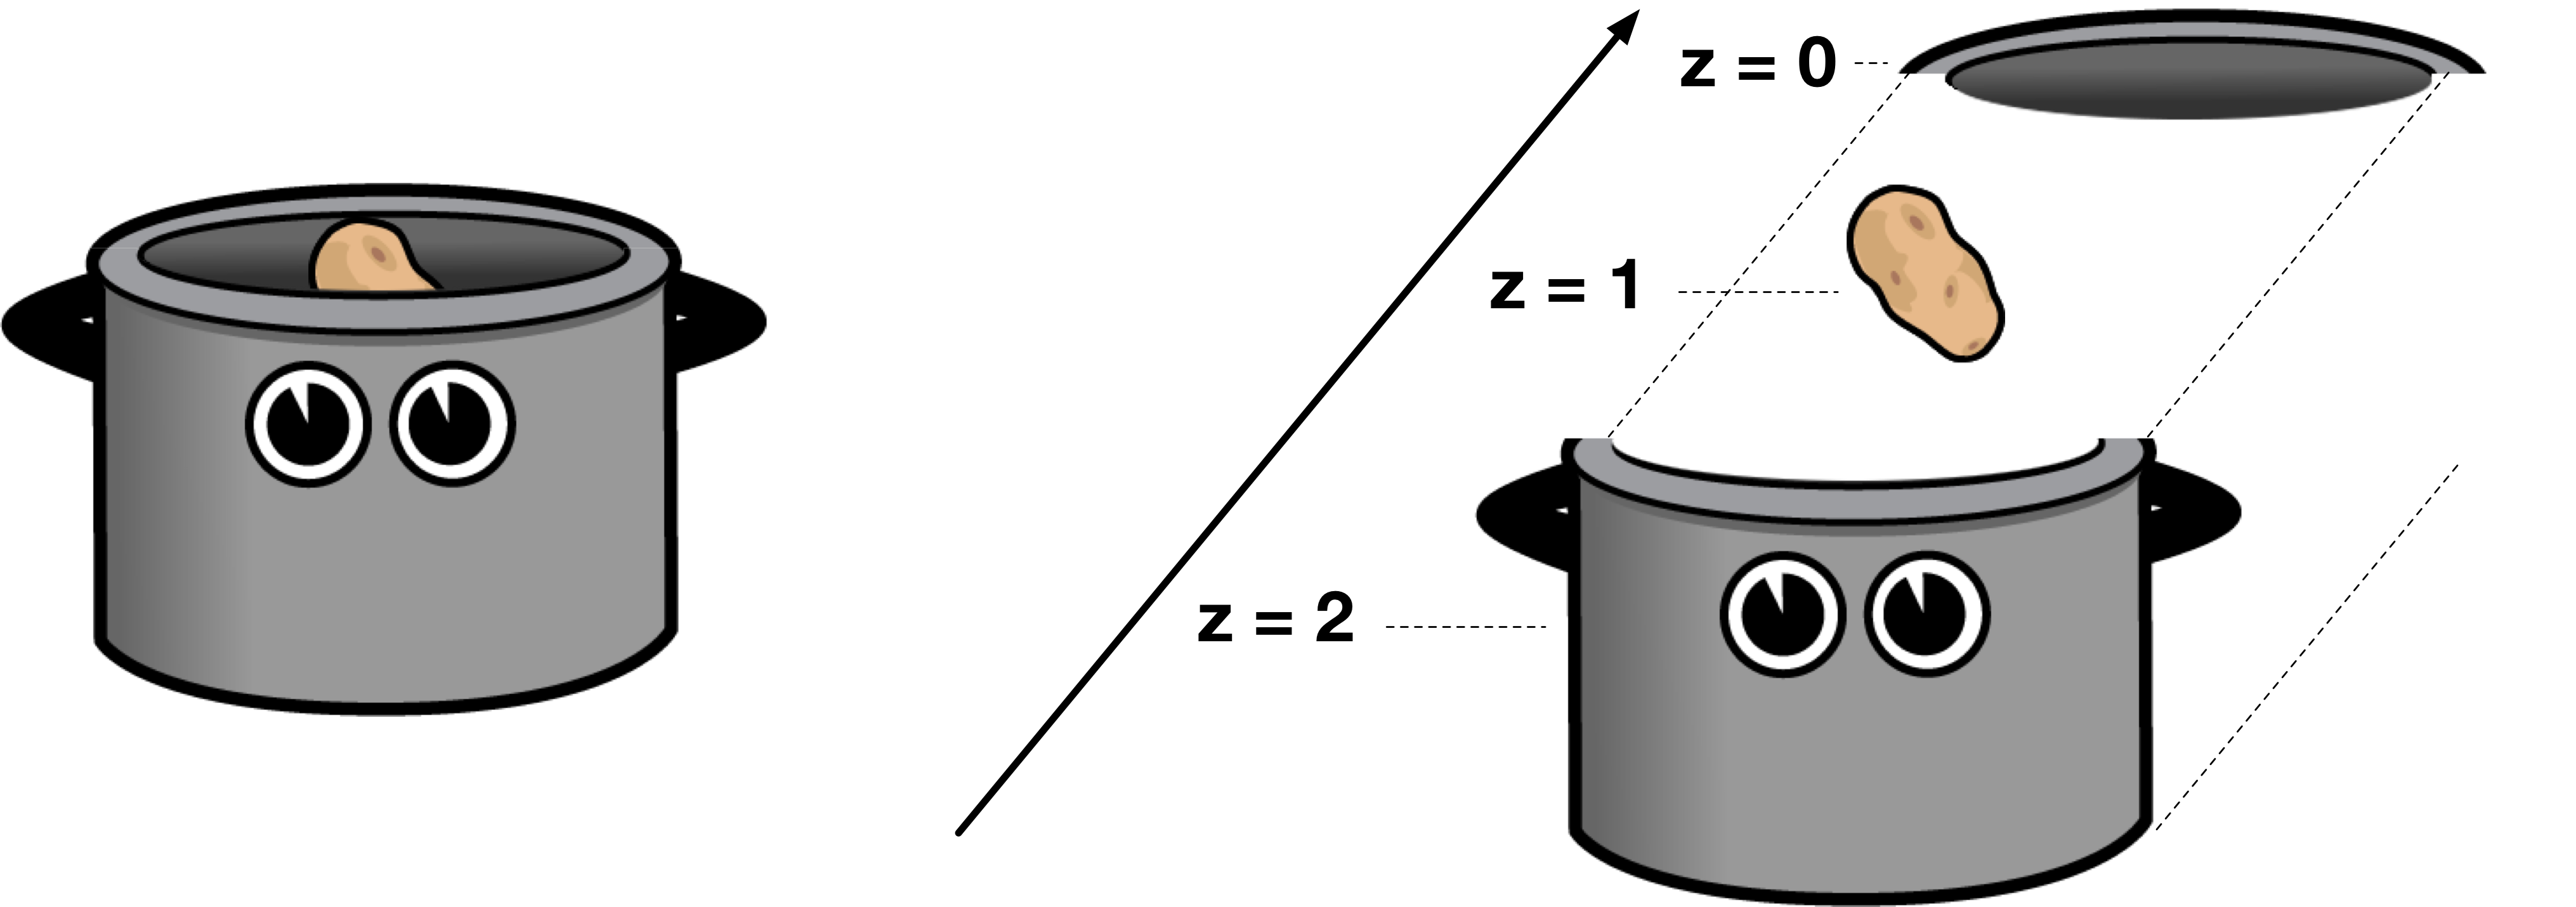
\includegraphics[width=0.9\linewidth]{images/Chapter3/drawing_order.png}
		\caption{Left: Objects on different Layers, Right: How the Z-Order influences
		on which Layer a node is rendered}
\end{figure}

For this solution to work all the falling objects and the bottom and top part of
our pot need to have the same parent node, otherwise we would not be able to use
the Z-Order to place the falling objects between the two parts of the pot. 

That is the reason why we are not creating a separate \ccbfile{} for the pot
object and instead place it inside of \inlinecode{MainScene.ccb}. There would be
other ways to work around this issue but adding the pot to the Main Scene is a
good solution for this game.

\begin{details}[frametitle={Global Z-order in \cocos{}}] 
While \cocos{} does not have support for global Z-order at the moment, it is
being discussed as a potential feature for future releases. Many games run into
issues as discussed above due to the lack of this feature. You can follow the
discussion on GitHub: \url{https://github.com/cocos2d/cocos2d-swift/issues/662}.
\end{details}

\subsection{Setting up the pot assets}
Equipped with everything we need to know about Z-order let's add the pot assets
to our Main Scene in \SB{}:

\begin{figure}[H]
		\centering
		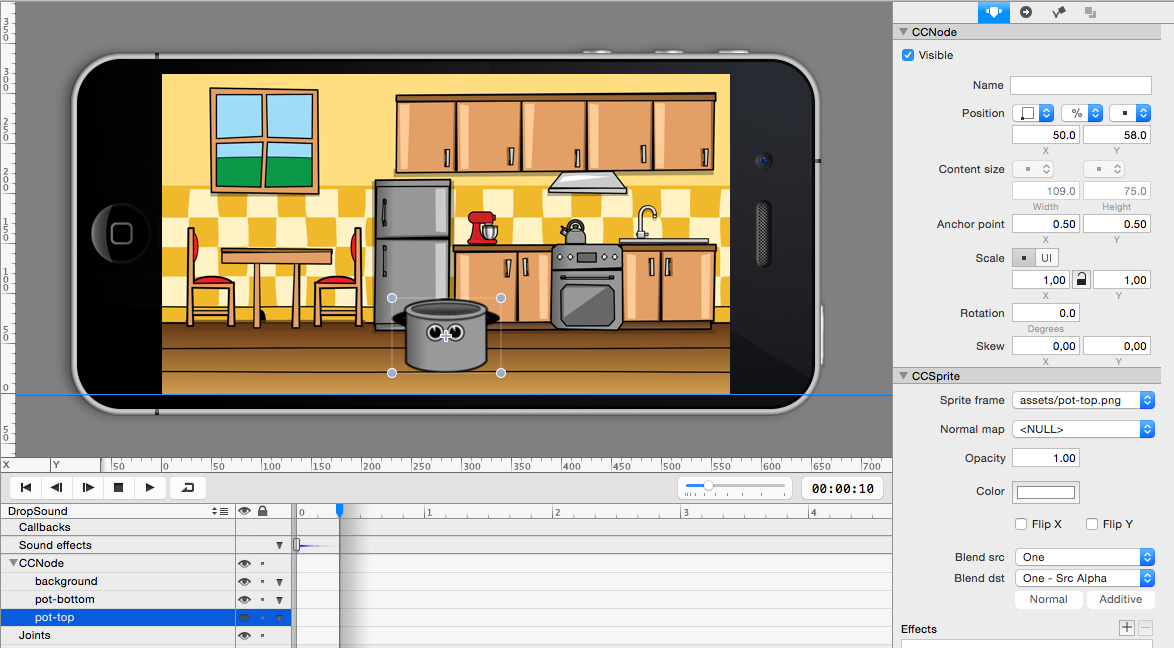
\includegraphics[width=0.9\linewidth]{images/Chapter3/add_pot.png}
		\caption{Add both pot parts to the main scene}
\end{figure}

\begin{leftbar}
The assets of both pot parts have exactly the same dimensions.
 Place both of them at 50\% X position and at a Y position of 58
Create code connections for both pot parts, linked to the \textit{Document Root}. 
Name them \inlinecode{potBottom} and \inlinecode{potTop} respectively.
Publish the \SB{} project
\end{leftbar}

Next, move to the \xcode{} project to set up the code connection variables and
implement the touch handling code.

\begin{leftbar}
Open \inlinecode{SBBMainScene.m} and add instance variables for our code
connections to the implementation block of \inlinecode{SBBMainScnene}:
\begin{lstlisting}
@implementation SBBMainScene {
    __weak CCSprite *_potTop;
    __weak CCSprite *_potBottom;
}
\end{lstlisting}
\end{leftbar}

Okay, now we have the basics set up and are ready to dive into the details of
implementing a drag and drop mechanism!

\section{Implement a Drag and Drop mechanism}
